% Created by tikzDevice version 0.10.1 on 2018-02-09 15:02:27
% !TEX encoding = UTF-8 Unicode
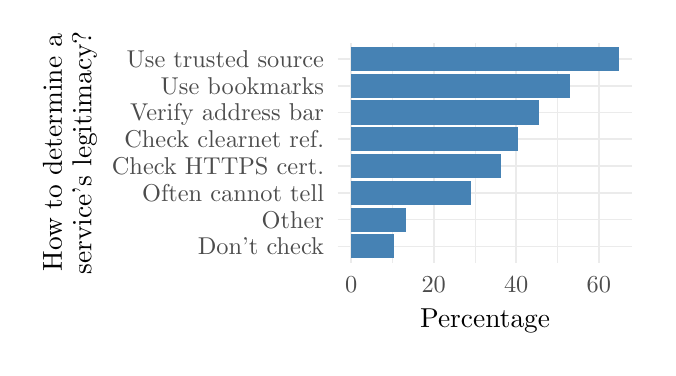
\begin{tikzpicture}[x=1pt,y=1pt]
\definecolor{fillColor}{RGB}{255,255,255}
\path[use as bounding box,fill=fillColor,fill opacity=0.00] (0,0) rectangle (224.04,115.63);
\begin{scope}
\path[clip] (112.04, 30.77) rectangle (218.54,110.13);
\definecolor{drawColor}{gray}{0.92}

\path[draw=drawColor,line width= 0.3pt,line join=round] (131.80, 30.77) --
	(131.80,110.13);

\path[draw=drawColor,line width= 0.3pt,line join=round] (161.62, 30.77) --
	(161.62,110.13);

\path[draw=drawColor,line width= 0.3pt,line join=round] (191.45, 30.77) --
	(191.45,110.13);

\path[draw=drawColor,line width= 0.6pt,line join=round] (112.04, 36.58) --
	(218.54, 36.58);

\path[draw=drawColor,line width= 0.6pt,line join=round] (112.04, 46.26) --
	(218.54, 46.26);

\path[draw=drawColor,line width= 0.6pt,line join=round] (112.04, 55.94) --
	(218.54, 55.94);

\path[draw=drawColor,line width= 0.6pt,line join=round] (112.04, 65.61) --
	(218.54, 65.61);

\path[draw=drawColor,line width= 0.6pt,line join=round] (112.04, 75.29) --
	(218.54, 75.29);

\path[draw=drawColor,line width= 0.6pt,line join=round] (112.04, 84.97) --
	(218.54, 84.97);

\path[draw=drawColor,line width= 0.6pt,line join=round] (112.04, 94.65) --
	(218.54, 94.65);

\path[draw=drawColor,line width= 0.6pt,line join=round] (112.04,104.33) --
	(218.54,104.33);

\path[draw=drawColor,line width= 0.6pt,line join=round] (116.88, 30.77) --
	(116.88,110.13);

\path[draw=drawColor,line width= 0.6pt,line join=round] (146.71, 30.77) --
	(146.71,110.13);

\path[draw=drawColor,line width= 0.6pt,line join=round] (176.53, 30.77) --
	(176.53,110.13);

\path[draw=drawColor,line width= 0.6pt,line join=round] (206.36, 30.77) --
	(206.36,110.13);
\definecolor{fillColor}{RGB}{70,130,180}

\path[fill=fillColor] (116.88, 32.22) rectangle (132.50, 40.93);

\path[fill=fillColor] (116.88, 41.90) rectangle (136.54, 50.61);

\path[fill=fillColor] (116.88, 51.58) rectangle (160.24, 60.29);

\path[fill=fillColor] (116.88, 61.26) rectangle (171.21, 69.97);

\path[fill=fillColor] (116.88, 70.94) rectangle (177.28, 79.65);

\path[fill=fillColor] (116.88, 80.61) rectangle (184.80, 89.32);

\path[fill=fillColor] (116.88, 90.29) rectangle (195.79, 99.00);

\path[fill=fillColor] (116.88, 99.97) rectangle (213.70,108.68);
\end{scope}
\begin{scope}
\path[clip] (  0.00,  0.00) rectangle (224.04,115.63);
\definecolor{drawColor}{gray}{0.30}

\node[text=drawColor,anchor=base east,inner sep=0pt, outer sep=0pt, scale=  0.88] at (107.09, 33.55) {Don't check};

\node[text=drawColor,anchor=base east,inner sep=0pt, outer sep=0pt, scale=  0.88] at (107.09, 43.23) {Other};

\node[text=drawColor,anchor=base east,inner sep=0pt, outer sep=0pt, scale=  0.88] at (107.09, 52.91) {Often cannot tell};

\node[text=drawColor,anchor=base east,inner sep=0pt, outer sep=0pt, scale=  0.88] at (107.09, 62.58) {Check HTTPS cert.};

\node[text=drawColor,anchor=base east,inner sep=0pt, outer sep=0pt, scale=  0.88] at (107.09, 72.26) {Check clearnet ref.};

\node[text=drawColor,anchor=base east,inner sep=0pt, outer sep=0pt, scale=  0.88] at (107.09, 81.94) {Verify address bar};

\node[text=drawColor,anchor=base east,inner sep=0pt, outer sep=0pt, scale=  0.88] at (107.09, 91.62) {Use bookmarks};

\node[text=drawColor,anchor=base east,inner sep=0pt, outer sep=0pt, scale=  0.88] at (107.09,101.29) {Use trusted source};
\end{scope}
\begin{scope}
\path[clip] (  0.00,  0.00) rectangle (224.04,115.63);
\definecolor{drawColor}{gray}{0.30}

\node[text=drawColor,anchor=base,inner sep=0pt, outer sep=0pt, scale=  0.88] at (116.88, 19.76) {0};

\node[text=drawColor,anchor=base,inner sep=0pt, outer sep=0pt, scale=  0.88] at (146.71, 19.76) {20};

\node[text=drawColor,anchor=base,inner sep=0pt, outer sep=0pt, scale=  0.88] at (176.53, 19.76) {40};

\node[text=drawColor,anchor=base,inner sep=0pt, outer sep=0pt, scale=  0.88] at (206.36, 19.76) {60};
\end{scope}
\begin{scope}
\path[clip] (  0.00,  0.00) rectangle (224.04,115.63);
\definecolor{drawColor}{RGB}{0,0,0}

\node[text=drawColor,anchor=base,inner sep=0pt, outer sep=0pt, scale=  0.99] at (165.29,  7.44) {Percentage};
\end{scope}
\begin{scope}
\path[clip] (  0.00,  0.00) rectangle (224.04,115.63);
\definecolor{drawColor}{RGB}{0,0,0}

\node[text=drawColor,rotate= 90.00,anchor=base,inner sep=0pt, outer sep=0pt, scale=  0.99] at ( 12.32, 70.45) {How to determine a};

\node[text=drawColor,rotate= 90.00,anchor=base,inner sep=0pt, outer sep=0pt, scale=  0.99] at ( 23.01, 70.45) {service's legitimacy?};
\end{scope}
\end{tikzpicture}
